\documentclass[a4paper,11pt]{jsarticle} 
%まず使用するパッケージ
\usepackage{amsmath, amsfonts, amssymb, mathtools, mathrsfs, latexsym}
%mathtoolsを用いたコマンド定義
\DeclarePairedDelimiter{\abs}{\lvert}{\rvert}
\usepackage{nccmath, empheq}

%\usepackage[draft]{graphicx}
\usepackage[dvipdfmx]{graphicx}
\usepackage[dvipdfmx]{color}
\usepackage{here, wrapfig, subcaption}
\usepackage{enumerate, comment, fancyhdr}
\usepackage{otf}

\usepackage{url}
\usepackage{otf}
\usepackage{fancyhdr}
\usepackage{seiritz}
\pagestyle{fancy}
  \cfoot{\thepage}
  \renewcommand{\headrulewidth}{0pt}

\begin{document}
%本文
\begin{titlepage}
  \hfill {最終更新日:\today}
  \begin{center}
    \vspace{\stretch{1}}
    {\Huge\gt テスト演習}\\ \vspace{\baselineskip}
    \textup{\large 実施日:2024年1月28日}\\ \vspace{\stretch{1}}
  \end{center}
  \vfill
  \begin{figure}[H]
    
\includegraphics[width=0.1\textwidth]{../images/qrcode.png}
  \end{figure}
\end{titlepage}

\qPart
%!TEX root = *.tex
%%%%%%%%%%%%%%%%%%
% カウンタのリセット
\setcounter{figure}{0}
% 問題文
{
\begin{wrapfigure}{r}{22zw}
  \vspace{-\intextsep}
  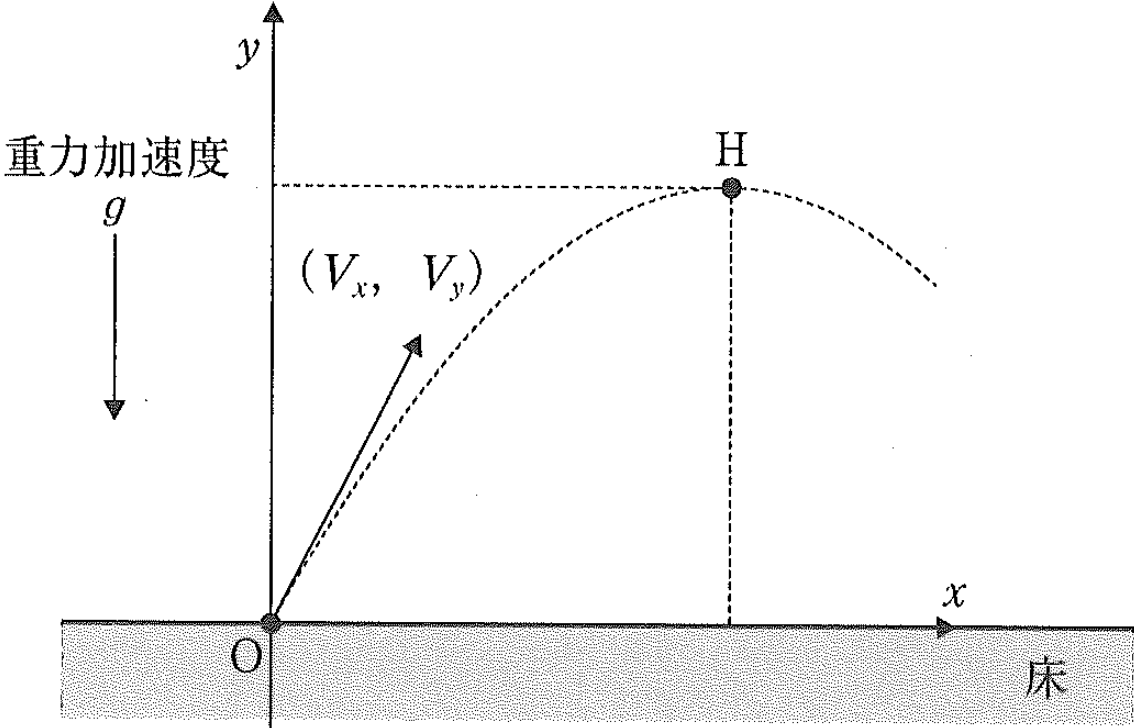
\includegraphics[width=22zw]{../graphs/noko_23_1.png}
  \caption{}
\end{wrapfigure}

なめらかで水平な床について,図1に示すように,原点Oおよび水平右向きに\x 軸,鉛直方向上向きに\y 軸を定める.
いま,質量$m$の小物体を原点Oから\xy 平面内において斜め上方に打ち出す.
この打ち出した瞬間の速度成分を,\x 方向,\y 方向それぞれについて$V_x$,$V_y$であるとする.
この小物体は鉛直下向きに一定の大きさ$mg$の重力を受けながら運動し,何度も床と衝突してはねかえる.
このとき,小物体と床の衝突は非弾性衝突であり,反発係数$e$は$0<e<1$である.
ただし,この小物体に対する空気抵抗は無視できるとする.
この小物体の運動について以下の問いに答えよ.
なお,解答において用いてよい文字は,特に指定がなければ$g,\,m,\,V_x,\,V_y$および$e$である.

\par}

\begin{enumerate}[(1)]
  \setlength{\leftskip}{-1zw}
  \setlength{\itemindent}{1zw}\setlength{\labelsep}{0.5zw}
  \setlength{\labelwidth}{1zw}\setlength{\leftmargin}{1zw}
  \setlength{\itemsep}{0.5\baselineskip}
  \item 小物体が打ち出されてから床と最初に衝突するまでの間における最高到達点Hの\x 座標,\y 座標をそれぞれ答えよ.
  \item 小物体が打ち出されてから床と最初に衝突する点を$\text{P}_1$とする.点$\text{P}_1$においてはねかえった直後の小物体の速度の\x 成分,\y 成分をそれぞれ答えよ.
  \item 点$\text{P}_1$における衝突において,小物体が失った力学的エネルギー$\varDelta E_1$を答えよ.
  \item 小物体が打ち出されてから床と2回目に衝突する点を$\text{P}_2$とする.点$\text{P}_2$における衝突において,小物体が失った力学的エネルギー$\varDelta E_2$を答えよ.
  \item 小物体が打ち出されてから床と$n$回目に衝突する点を$\text{P}_n$とする.点$\text{P}_n$における衝突において,小物体が失った力学的エネルギー$\varDelta E_n$を答えよ.ただし,この答えには,問題文はじめに指定した文字に加えて$n$を用いてよい.
  \item 小物体が打ち出されてから床と最初に衝突するまでの間における最高到達点Hの衝突回数が十分に大きくなると,小物体の衝突直後の速度は最終的に一定となる.この一定となった速度の\x 成分,\y 成分をそれぞれ答えよ.
  \item 小物体が打ち出されてから床と$n$回目に衝突するまでに失った力学的エネルギーの総和について考える.床との衝突回数が十分に大きくなると,この総和は最終的にある値となる.この値を答えよ.
\end{enumerate}





% メモ
\begin{comment}

\end{comment}


%%%%%%%%%%%%%%%%%%

\calcPage

\qPart
%!TEX root = *.tex
%%%%%%%%%%%%%%%%%%
% カウンタのリセット
\setcounter{figure}{0}
% 問題文

次の文章の$\BrankNo{(1)}\sim\BrankNo{(12)}$に適切な式を入れよ.
\BrankNo{(6)}以外の解答には,国際単位系(SI)に基づいた単位を併記せよ.
起電力$E_1\unit{V}$の直流電源,
起電力の実効値$E_2\unit{V}$の交流電源,
抵抗値の初期値が$R_1\unit{Ω}$である可変抵抗,
抵抗値$R_2\unit{Ω},\,R_3\unit{Ω}$の抵抗,
電気容量$C\unit{F}$の平行板コンデンサー,
自己インダクタンス$L\unit{H}$のコイル,
スイッチ$\text{S}_1,\,\text{S}_2$から成る図1の電気回路を考える.
$\text{S}_1$ははじめ開かれており,$\text{S}_2$は右側の接点をAとBのいずれかに切り替えるスイッチである.
コンデンサーの極板間は真空であり,極板間距離は$d\unit{m}$,真空の誘電率は$\epsilon_0\unit{F/m}$とする.
また,交流電源の角周波数は可変である.

\begin{enumerate}[問1.]
  \setlength{\leftskip}{-1zw}
  \setlength{\itemindent}{1zw}\setlength{\labelsep}{0.5zw}
  \setlength{\labelwidth}{1zw}\setlength{\leftmargin}{1zw}
  \setlength{\itemsep}{0.5\baselineskip}
  \item $\text{S}_2$をA側に閉じ,さらに$\text{S}_1$を閉じて十分に時間が経過した後,コンデンサーの極板間の電圧は\BrankNo{(1)}となる.このとき,コンデンサーに蓄えられている電荷量は\BrankNo{(2)},静電エネルギーは\BrankNo{(3)}と表すことができる.また,コイルの電磁エネルギーは\BrankNo{(4)}となる.
  \begin{enumerate}
    \setlength{\leftskip}{-2zw}
    \setlength{\itemindent}{1zw}\setlength{\labelsep}{0.5zw}
    \setlength{\labelwidth}{1zw}\setlength{\leftmargin}{1zw}
    \setlength{\itemsep}{0.5\baselineskip}
    \item[(ア)] ここで$\text{S}_1$を再び開いた場合,振動電流が収束するまでの間に失われるジュール熱は\BrankNo{(5)}と表される.
    \item[(イ)] $\text{S}_2$を閉じたまま,図2に示すように極板間に厚さ$d_0\unit{m}$,比誘電率$\epsilon_r$の誘電体を挿入すると,コンデンサーの電気容量は元の\BrankNo{(6)}倍となる.このとき,コンデンサーに蓄えられる電荷量を\BrankNo{(2)}とするためには,可変抵抗の大きさを\BrankNo{(7)}とすればよい.
  \end{enumerate}
  \item $\text{S}_1$を開き,コンデンサーに挿入した誘電体を取り外し,$\text{S}_2$をB側に切り替えて十分に時間が経過したものとする.
  抵抗値$R_3\unit{Ω}$の抵抗にかかる電圧と点D--F間にかかる電圧のそれぞれの実効値が等しいとき,
  交流電源の角周波数は\BrankNo{(8)},交流電源から供給される電流の実効値は\BrankNo{(9)}となる.
  この状態で1時間が経過する間に消費される電力量は\BrankNo{(10)}である.
  また,交流電源の角周波数を調整して\BrankNo{(11)}とすると,
  交流電源から供給される電流の実効値は最大となり,その値は\BrankNo{(12)}となる.
\end{enumerate}

\begin{figure}[htbp]
  \centering
  \begin{minipage}{.65\columnwidth}
    \centering
    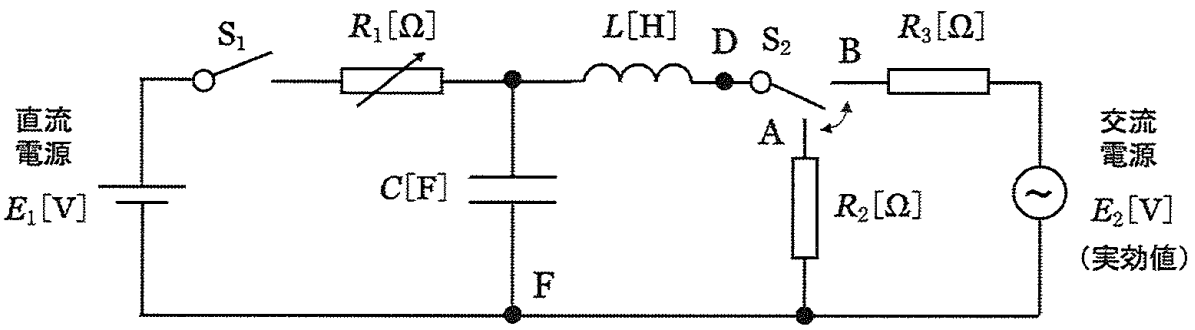
\includegraphics[width=\columnwidth]{../graphs/yokokoku_23_2-1.png}
    \caption{}
  \end{minipage}
  \begin{minipage}{.2\columnwidth}
    \centering
    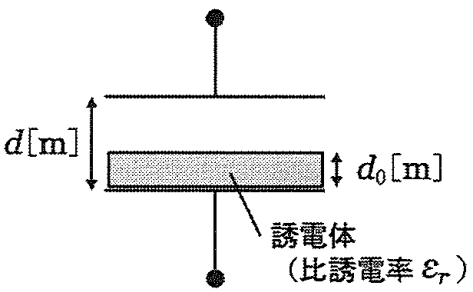
\includegraphics[width=\columnwidth]{../graphs/yokokoku_23_2-2.png}
    \caption{}
  \end{minipage}
\end{figure}


% メモ
\begin{comment}

\end{comment}


%%%%%%%%%%%%%%%%%%

\calcPage

\qPart
%!TEX root = *.tex
%%%%%%%%%%%%%%%%%%
% カウンタのリセット
\setcounter{figure}{0}
% 問題文
以下の文章中の$\BrankNo{(ア)}\sim\BrankNo{(ケ)}$に適切な式を記入しなさい.

図1のように,ピストン付きのシリンダーが大気中で水平な台の上に置かれている.
ピストンの厚さは無視でき,その質量は$M$で,断面積は$S$である.
シリンダーの内部には,物質量1モルの単原子分子からなる理想気体が閉じ込められている.
シリンダー内壁には,小さなストッパーA,Bがシリンダー内側の底面から高さ$L,\,\tfrac{5}{3}L$の位置にそれぞれ取り付けられており,
ピストンはその間を傾かずになめらかに動く.
ピストンの上側には,質量の無視できるフックが取り付けられている.
また,シリンダー内には体積の無視できる加熱冷却器が設置されており,
理想気体を加熱・冷却できる.
ピストンとシリンダーは断熱材でできており,
加熱冷却器以外では,シリンダー内の理想気体と外部の間に熱の移動はない.
大気圧を$p_0$,重力加速度の大きさを$g$,気体定数を$R$とする.

\hang{(1)}
図1のように,はじめピストンはストッパーAの上に置かれており,シリンダー内の理想気体の圧力は大気圧と同じ$p_0$であった.
このときの理想気体の温度(絶対温度)は$\BrankNo{(ア)}$であった(状態1).
シリンダー内の理想気体を加熱冷却器でゆっくり加熱したところ,
その圧力が\BrankNo{(イ)}に達したとき(状態2),ピストンは上昇をはじめた.
状態1→状態2の過程で,理想気体の内部エネルギーは\BrankNo{(ウ)}だけ増加した.
さらに過熱を続けたところ,ピストンは,理想気体の圧力を(イ)に保ったままゆっくりと上昇し,
やがてストッパーBに到達した(状態3).
状態2→状態3の過程で,理想気体が外部にした仕事は\BrankNo{(エ)}であった.
また状態2→状態3の過程で,加熱冷却器から理想気体に加えられた熱量は\BrankNo{(オ)}であった.

\hang{(2)}
図2のように,ばね定数$k$のばねの一方の端をピストンに取り付けたフックに固定し,
他端を天井に固定した.
加熱冷却器で理想気体の温度を調整し,その圧力を大気圧と同じ$p_0$にした.
このとき,ピストンはストッパーBの位置で静止しており,
ばねは自然長から$\tfrac{1}{3}L$だけ伸びていた(状態4).
状態4から理想気体を冷却したところ,理想気体の温度(絶対温度)が\BrankNo{(カ)}に達したとき(状態5),ピストンは下降をはじめた.
状態4→状態5の過程で加熱冷却器が理想気体から吸収した熱量は\BrankNo{(キ)}であった.
さらに冷却を続けたところ,ピストンは,力のつりあいを保ちながらゆっくりと下降し,
やがてストッパーAに到達した(状態6).
このときの理想気体の圧力は\BrankNo{(ク)}であった.
圧力--体積グラフ($p$--$V$グラフ)を考えると,
状態5→状態6の過程で理想気体が外部にした仕事は\BrankNo{(ケ)}であった.

\begin{figure}[H]
  \centering
  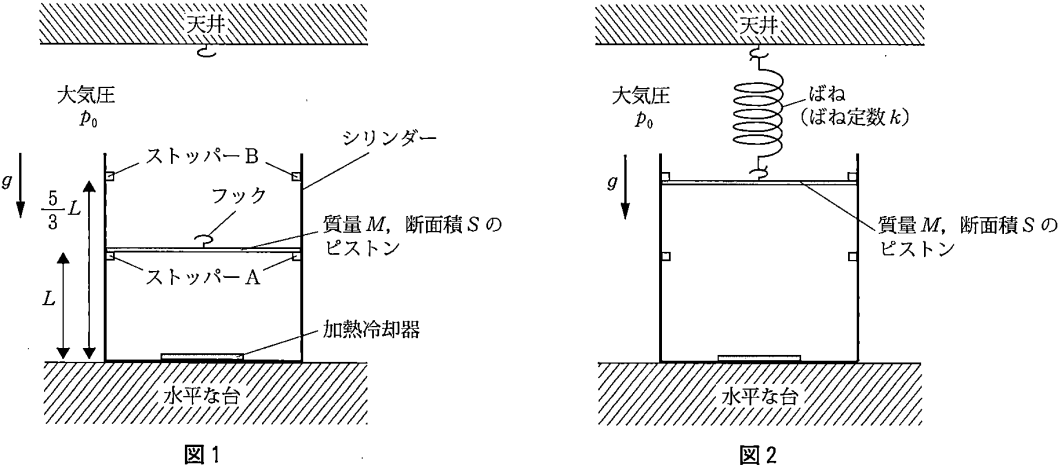
\includegraphics[width=\columnwidth]{../graphs/ko_riko_23_3.png}
\end{figure}


% メモ
\begin{comment}

\end{comment}


%%%%%%%%%%%%%%%%%%

\clearpage

\brankPage

\end{document}

